\documentclass[../Analysis-3.tex]{subfiles}

\begin{document}
\chapter*{Lecture 26} %Set chapter name
\addcontentsline{toc}{chapter}{Lecture 26} %Set chapter title
\setcounter{chapter}{26} %Set chapter counter
\setcounter{section}{0}
\setcounter{equation}{0}
\setcounter{figure}{0}


\section{Examples}
Recall in previous lecture, we discussed how to find area of a surface over a bounded region. Now we will look towards some examples.

\begin{Eg}{Truncated Cylinder}{}\index{Truncated Cylinder}

  \begin{wrapfigure}{r}{0.40\textwidth}
    \centering
    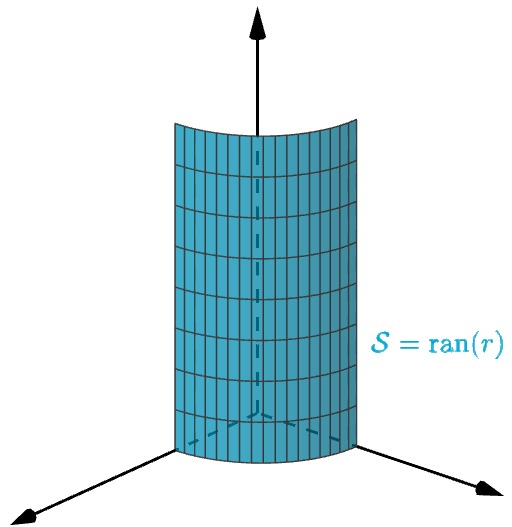
\includegraphics[width=.78\linewidth]{../figures/lec-26.1.png}
    \caption{Truncated Cylinder}
  \end{wrapfigure}

  Let $\mathcal{R} \subseteq \R^2$ be a region. $r : \mathcal{R} \to \R^3$ be a map defined by $r(x,y) = (\cos(x),\sin(x),y)$. Here the region is given by,
  \[\mathcal{R} = \{(x,y) \mid 0 \le x \le \frac{\pi}{2}, 0\le y \le 1\} = \qty[0,\frac{\pi}{2}] \times [0,1] \]

  It can be seen easily that $r$ is parametrization of a surface $\ran(r) = \mathcal{S}$. We want to calculate the surface area of it.

  For this case, $r_x = (-\sin x, \cos x, 0)$ and $r_y =(0,0,1)$. So, $ r_x \times r_y = (\cos x, \sin y, 0)$ and hence, $\norm{r_x \times r_y} = 1$. Therefore,

  $\displaystyle \Area(\mathcal{S}) = \int_{\mathcal{R}} 1 \dd A = \int_0^{\frac{\pi}{2}} \int_{0}^1 1 \dd A = \frac{\pi}{2}$

\end{Eg}


\begin{Eg}{Hemisphere}{}\index{Hemisphere}

  \begin{wrapfigure}{r}{0.45\textwidth}
    \centering
    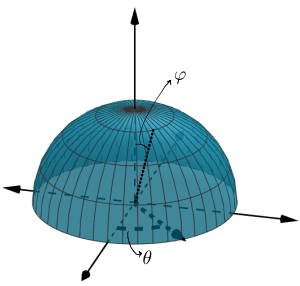
\includegraphics[width=.78\linewidth]{../figures/lec-26.2.png}
    \caption{Hemisphere}
  \end{wrapfigure}

  $\mathcal{S} = \qty{(x,y,z) \mid x^2+y^2+z^2 = 1, z >0 }$ is a surface. This surface actually surface of unit Hemisphere.

  Parametrization of the surface $\mathcal{S}$ is given by, $r(\theta, \varphi) = (\cos \theta \cos \varphi, \sin \theta \cos \varphi, \sin \varphi)$ where, $0 \le \varphi \le \frac{\pi}{2}, 0 \le \theta \le 2\pi$. So,

  \begin{align*}
    r_{\theta}                                    & = (-\sin \theta \cos \varphi, \cos \theta \cos \varphi, 0)                              \\
    r_{\varphi}                                   & = (-\cos \theta \sin \varphi,-\sin \theta \sin \varphi, \cos \varphi)                   \\
    \therefore r_{\theta} \times r_{\varphi}      & = (\cos \theta \cos ^2 \varphi, \sin \theta \cos ^2\varphi, \cos \varphi  \sin \varphi) \\
    \implies \norm{r_{\theta} \times r_{\varphi}} & = \cos \varphi
  \end{align*}

  Hence, $\displaystyle\Area(\mathcal{S}) = \int_{0}^{\frac{\pi}{2}}\int_{0}^{2\pi} \cos \varphi\, \dd \theta \dd \varphi = 2\pi$

\end{Eg}

\section{Surface Integral over Scalar fields}\index{Surface Integral}

Let, $\mathcal{R} \in \R^2$ be a region. $r:\mathcal{R} \to \R^3$ be parametrization of a surface $\mathcal{S}$. $f$ be a scalar function defined on the surface $\mathcal{S}$. Let $f \in C(\mathcal{S})$ then we can define integration of $f$ over the surface as following,

\begin{align}
  \int_{\mathcal{S}} f \, \dd \mathcal{S}
   & := \lim_{\norm{\mathcal{P}} \to 0} \sum_{\alpha \in \Lambda (\mathcal{P})} f(r(x_{\alpha})) \norm{r_u(x_{\alpha}) \times r_v(x_{\alpha})} \Area(B_{\alpha}^2) \nonumber \\
   & = \int_{\mathcal{R}} (f \circ r)(u,v) \norm{r_u \times r_v} \, \dd A \label{eq:siovf}
\end{align}

As we have noticed in the case of \textbf{Line Integral of over a scalar field} the integration do not depend on the parametrization of the path. In this case also if we have different two parametrization $r, \tilde{r}$ for the surface $\mathcal{S}$ then there exist a one-one continuous function $\varphi$ so that the following diagram commutes, (in other words $r = \tilde{r} \circ \tilde{\varphi}$)

\[\begin{tikzcd}
    & {\mathcal{S}} \\
    {\mathcal{R}} && {\tilde{\mathcal{R}}}
    \arrow["r", from=2-1, to=1-2]
    \arrow["{\tilde{r}}"', from=2-3, to=1-2]
    \arrow["\varphi"', from=2-1, to=2-3]
  \end{tikzcd}\]

We can show that the integration in (\ref{eq:siovf}) is also same if we replace $r$ by $\tilde{r}$. In other words the surface Integral over a surface is independent of its parametrization (See Figure \ref{Examp:1}).

\begin{Eg}{Surface Integral over a Cone}{surf:int:o:cone}
  We want to evaluate \[ \int_{\mathcal{S}}(x^2+y^2+z^2) \dd \mathcal{S}\]

  where, $\mathcal{S} = \qty{(x,y,z) \mid z = \sqrt{x^2 + y^2},0 \le z \le 1}$

  \textit{Solution.} Let,$\mathcal{R} = \qty{(x,y)| x^2+y^2 \le 1}$ be the region and $r(x,y) = \left( x,y,\sqrt{x^2+y^2} \right)$ is the parametrization of the surface $\mathcal{S}$. Here, $r_x = \left( 1,0, \frac{x}{\sqrt{x^2+y^2}} \right)$ and $r_y = \left( 0,1,\frac{y}{\sqrt{x^2+y^2}} \right)$.


  \begin{align*}
    \therefore \int_{\mathcal{S}}(x^2+y^2+z^2) \, \dd \mathcal{S}
     & = \int_{\mathcal{R}} (f\circ r) \cdot \norm{r_x \times r_y} \, \dd A                                           \\
     & = \int_{\mathcal{R}} (f\circ r) \sqrt{1 + \frac{x^2}{x^2+y^2} + \frac{y^2}{x^2+y^2}} \, \dd A                  \\
     & = 2\sqrt{2} \int_{\mathcal{R}} (x^2+y^2) \, \dd A                                                              \\
     & = 2\sqrt{2} \int_{0}^{1} \int_{0}^{2\pi} r^3 \, \dd \theta \, \dd r \quad (\text{It's the polar substitution}) \\
     & = \sqrt{2} \pi
  \end{align*}

\end{Eg}

\section{Surface Integral over a Vector field}\index{Surface Integral}

Let $\vec{F} : \mathcal{S} \to \R^3$ be a vector field defined on a surface $\mathcal{S}$. We want to calculate the flux of $\vec{F}$ over the surface $\mathcal{S}$.

\begin{tcolorbox} \label{Examp:1}

  \begin{wrapfigure}{r}{0.50\textwidth}
    \centering
    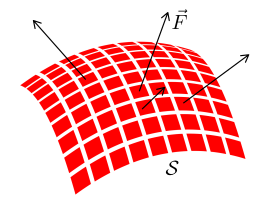
\includegraphics[width=.78\linewidth]{../figures/lec-26.3.png}
    \caption{A surface with Vector field}
  \end{wrapfigure}

  Let $\mathcal{S}$ be a surface and $\vec{F}$ (This function is $C^1$ over $\mathcal{S}$) be the Vector field defined over it. We can assume $\vec{F}$ to be a force. We want to compute the extent to which $\vec{F}$ is pushing the surface along normal to $\mathcal{S}$. In other words, we want to calculate \textbf{Flux / Flow} of $\vec{F}$ through $\mathcal{S}$.

  \

  Let $\dd S$ be a tiny part of  this surface. Flux\index{Flux} through $\dd S$ is given by $\vec{F}\cdot\vec{n}\, \dd S$ where, $\vec{n}$ is the unit normal vector through the surface at a point $x \in \dd S$. Since $\dd S$ is small enough we can assume $\vec{n}$ is almost constant over $\dd S$. So, the total flux must be

  \[ \textbf{Flux} = \int_{\mathcal{S}} \vec{F}\cdot\vec{n}\, \dd S \]

  But, there is a problem! If the surface $\mathcal{S}$ has a point where two normal vectors with different direction are the at same point then the concept of flux does not make any sense. That's why we have to come up with some conditions. Namely, \textit{Orientation of Surface}.

\end{tcolorbox}

So we formalize the notion of ``Orientation''\index{Orientation} with the following definition. Thought it is only for the surfaces in $ \R^3 $. Later in Differential Geometry, you will see this notion in a more general way (for manifolds).

\begin{Def}{Oriented Surface}{orient:surf}\index{Oriented Surface}
  A surface is \textbf{oriented} if there exists a continuous function $\vec{n} : \mathcal{S} \to \R^3$ such that $\vec{n}(x)$ is normal to $\mathcal{S}$ at the point $x$ and $\norm{\vec{n}(x)} = 1$.
\end{Def}

Surfaces like \textbf{Möbius strip} or \textbf{Klein Bottle} are not oriented.

\begin{Def}{Surface Integral over Vector field}{}
  Let, $\mathcal{S}$ be an oriented surface with normal vector $\vec{n}$ and $\vec{F} : \mathcal{S} \to \R^3$ be a $C^1$ vector field defined over $\mathcal{S}$. Then the ``Surface Integral'' of $\vec{F}$ over $\mathcal{S}$ is defined as following,
  \[ \int_{\mathcal{S}} \vec{F} \cdot \dd \vec{S} = \int_{\mathcal{S}} \vec{F}\cdot\vec{n}\, \dd S \]
\end{Def}


\end{document}
